\subsection{Optical Receiver Device}
\label{TOORD}
The main objective of the \ac{ORD} is to detect the individual energy quanta. A large fraction of the photons emitted by the \acs{laser} are not that easy for detection since they are redirected by the atmosphere, spread due to surface scattering or they are simply absorbed partly by either of them. The decrease in photon quantity is really severe considering these factors and that is why a photon detector with comparable high quantum efficiency is required. Since the number of photons actually reaching the perimeter of the \ac{ORD} is usually only in the order of one to ten, the \acs{ORD} has to be able to detect and analyze individual small energy packets, preferably single photons. In this section, general introduction about photon detection is drawn first, then the \acs{laser} wavelength estimation is performed to narrow down wavelength range.After that design option tree is pruned according to the wavelength requirement and technology availability, and there are new approaches after deeply research. Finally the trade off is performed which is split up into trade method, trade criteria and weight factor, followed by trade off summary. The design selection for the optical receiver device is done at the end of the section.

\subsubsection{General Introduction to Photon Detection}
\label{introReceiver}
Photon detection typically occurs in a two-step process: the absorbed photon creates a measurable change in the detector's electrical properties, and the changes is registered in an external read-out integrated circuit (\acs{ROIC}). In general, the detector material responds either \textit{directly} to the incident photon by generating a free charge, with this charge then being responsible for producing the change in electrical properties, or \textit{indirectly}, with the absorbed optical power generating a temperature rise in the detector material, which is responsible for producing the change in electrical properties. In either case, this photon-induced analog signal is registered and amplified in the \acs{ROIC} digitization for further signal processing. 

Additional factors include the detector material \textit{sensitivity} and the detector \textit{device speed of response}. Sensitivity is a measure of how few photons are required to raise the detector output above any background noise level present in the absence of incident light. Response speed is a measure of how faithfully the detector's electrical output responds to changes in the intensity of the input light signal.

\subsubsection{Solide-State Photon Detection}
\label{ssphotonsensing}
Solid-state imaging is based on the physical principle of converting light (photons) into a measurable quantity (electrical voltage, electrical current). Photons falling onto and penetrating into a semiconductor substrate can transfer part of their energy to the substrate by generating electron-hole pairs. For an n-type semiconductor, if the energy content of the photons is high enough, electrons can be released from the valence band and swept into the conduction band, leaving behind a hole in the valence band. To generate an electron-hole pair, the energy of the photons has to be larger than the bandgap of the semicondector substrate.\cite{photogrammetry}

For reasons of cost and miniaturization, a solid state solution for single photon detection is highly desirable. Figure \ref{fig:intro_receiver1} on page \ref{fig:intro_receiver1} shows a classification that covers the current state-of-the-art on optical solid-state 3D image sensors. 

\begin{figure}
\centering
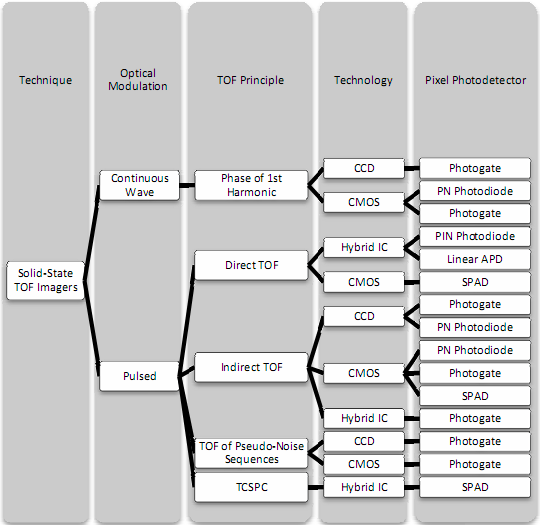
\includegraphics[scale = 1]{chapters/img/intro_receiver1.png}
\caption{Classification of state-of-the-art optical TOF image sensors.}
\label{fig:intro_receiver1}
\end{figure}

\subsubsection{\acs{SPAD}}
\label{SPAD}
\ac{SPAD} are solid-state semiconductor devices based on a p-n junction reversed biased at a voltage $V_{a}$ higher than $V_{B}$.

\begin{figure}
\centering
\includegraphics[scale = 1]{chapters/img/SPAD_Cross-section.png}
\caption{\acs{SPAD} cross-section diagram.}
\label{fig:SPAD_cross-section}
\end{figure}

At this bias, the electric field is so high (higher than 3��105 V/cm) that a single charge carrier injected in the depletion layer can trigger a self-sustaining avalanche. The current rises swiftly (sub nanosecond rise-time) to a macroscopic steady level, in the milliampere range. If the primary carrier is photo-generated, the leading edge of the avalanche pulse marks (with picoseconds time jitter) the arrival time of the detected photon. The current continues until the avalanche is quenched by lowering the bias voltage VD down to or below $V_{B}$: the lower electric field is not able any more to accelerate the carriers to impact-ionize with lattice atoms, therefore current ceases. In order to be able to detect another photon, the bias voltage must be raised again above breakdown.\cite{SPAD_intro}

\subsubsection{Wavelength estimation}
\label{introReceiver}
Laser wavelength is one of the most important parameters influencing the whole design of photon detection device and \acs{laser} emitter choosing. Different emitter wavelengths have different photon detection efficiency or probability to photon receiver. To choose which type of \acs{laser} is feasible, it is best to start with which wavelength the receiver can detect.

According to the photon detection probability distribution diagram for \acs{SPAD} and \acs{MPD} in figure \ref{fig:SPAD_efficiency} and \ref{fig:MPD_efficiency} on page \ref{fig:SPAD_efficiency} and \ref{fig:MPD_efficiency}, the general most sufficient wavelength range is between 400nm to 900nm. 

\begin{figure}
\centering
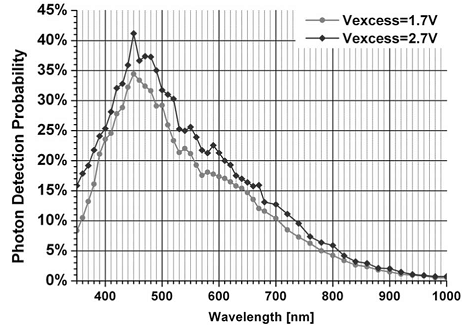
\includegraphics[scale=1]{chapters/img/SPAD_efficiency.png}
\caption{\acs{SPAD} photon detection probability as a function of wavelength for two values of excess bias voltage}
\label{fig:SPAD_efficiency}
\end{figure}

\begin{figure}
\centering
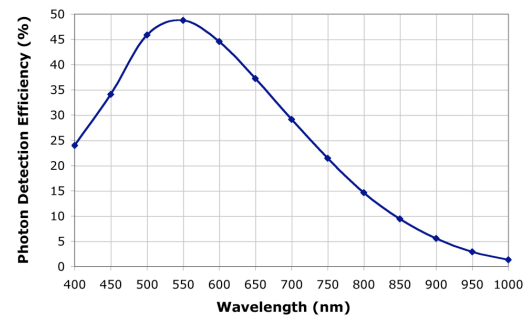
\includegraphics[scale=1]{chapters/img/MPD_efficiency.png}
\caption{\acs{MPD} photon detection probability as a function of wavelength}
\label{fig:MPD_efficiency}
\end{figure}

There are not much qualified \acs{laser}s can be considered below the wavelength 400nm, and the photon detection probability is insufficient if the wavelength go above 900nm. In order to narrow the wavelength range, the atmospheric transmittance versus photon detection efficiency ratio is introduced, which means that larger ratio indicates larger chance the receiver can detect photon. The actual formula to calculate the ratio is R = transmittance$^{2} \times$ photon efficiency. The transmittance is squared because the light go through the atmosphere twice. Calculate all ratio between wavelength 400nm to 900nm by interval 25nm, and plot the ratios in figure \ref{fig:wavelength_estimation} on page \ref{fig:wavelength_estimation}. From the graph, it is easy to narrow down the wavelength range to 425nm-500nm.  The following sections will give brief trade-offs between \acs{laser} emitters and receivers.

\begin{figure}
\centering
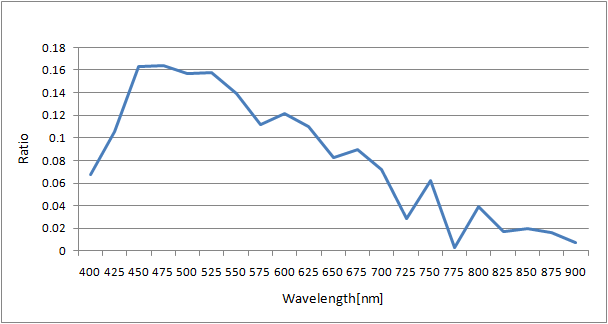
\includegraphics[scale=1]{chapters/img/wavelength_estimation.png}
\caption{Ratio of atmospheric transmittance versus photon detection efficiency}
\label{fig:wavelength_estimation}
\end{figure}


\subsubsection{Receiver Prune}
\label{TOReceiverP}
In the design option tree, the GLAS branch is obviously dropped out, since we are trying to improve the whole concept. Meanwhile, the \ac{MPD}'s single-photon detection modules branch has different quantum efficiency for different wavelength. Which means MPD can be a good option for the blue laser detector with 35\% efficiency. The \ac{SPAD} chip could be an approach since it has reasonable high quantum detect efficiency at laser wavelength 425nm to 475nm. Both \acs{MPD} and \acs{SPAD} are not optimal for \acs{NIR} or \acs{IR} laser detect with low quantum efficiency around 1\%. 

The pruned design option tree for the laser detector can be seen in figure \ref{fig:PrunedReceiver} on page \ref{fig:PrunedReceiver}.

\begin{figure}
\centering
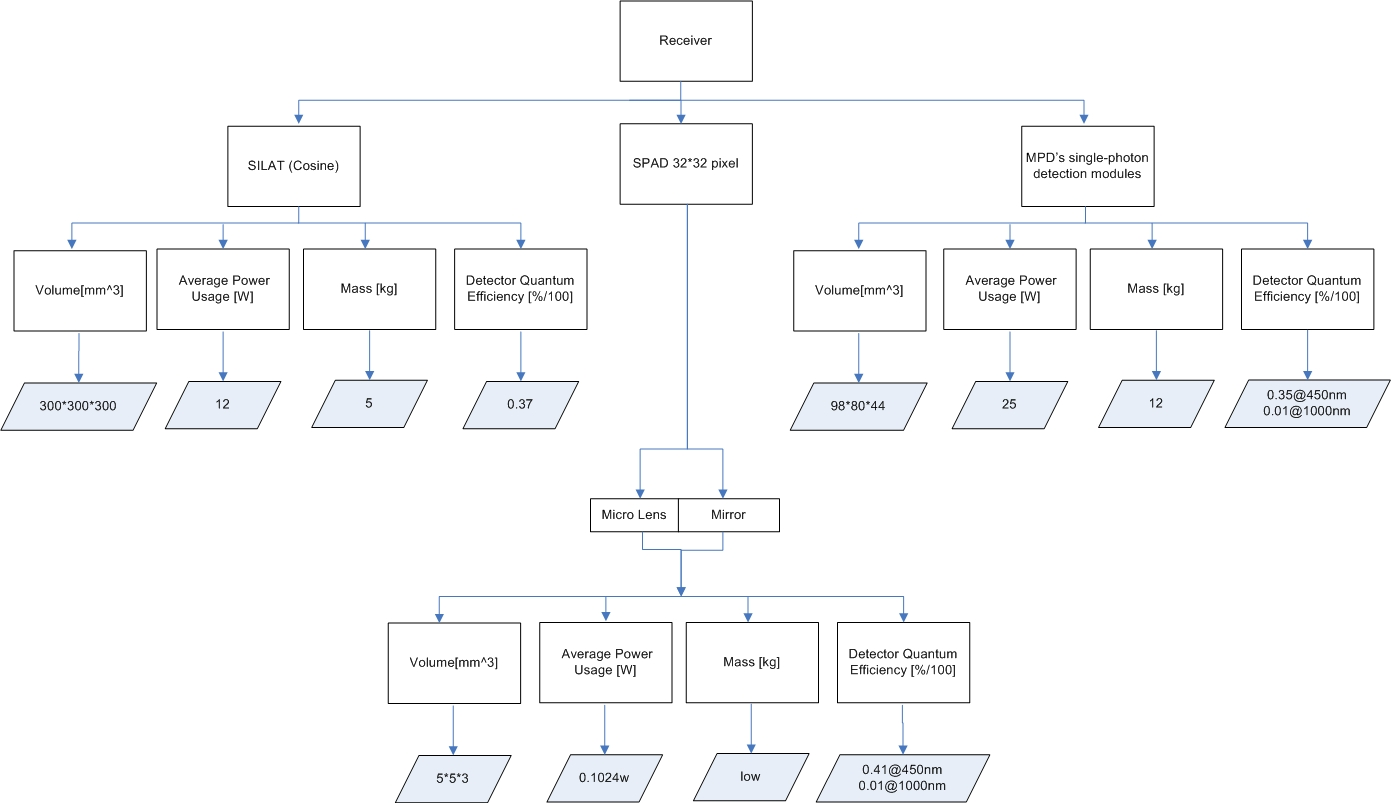
\includegraphics[scale=0.7, angle=90]{chapters/img/DOTreceiverPruned.jpg}
\caption{The pruned design option tree for the Laser receivers}
\label{fig:PrunedReceiver}
\end{figure}

\subsubsection{Trade Method}
\label{TOReceiverM}
There are mainly four options after pruning and each have different strong points or weak points. 

The first option is \ac{SILAT}, which combines two optical cameras with a low-power photon-counting laser altimeter. It means that \acs{SILAT} operates both pulse laser and photon detector, and it need to be configured as only a photon detector(more information are needed about the configuration). The main strong point is that \acs{SILAT} should has relative higher reliability since it is designed suitable for space mission like spectral imagery and satellite topographic study. 

\ac{MPD}'s photon detection efficiency is obtained through the use of epitaxial silicon \ac{SPAD} and patented \ac{IAQC}, which is specifically designed and optimized for photon counting. The main drawback is that it is difficult to achieve the precise ground resolution due to diffraction.

The final option is use a 32*32 pixel array with in-pixel photon counting, which also use \acs{SPAD} but in \ac{CMOS} technology. It has the highest quantum efficiency for blue laser(@450nm), but only 2\% of the chip area can detect the quanta. In this case, micro lenses or faceted mirrors are used in order to collect most of the incoming quanta focus on such a small area. The solution is shown in figure \ref{fig:diagram_Rgeneral} on page \ref{fig:diagram_Rgeneral}. The parabolic mirror is placed at certain position to the small \acs{SPAD} chip with specified curvature, then the prism barrier is designed to filter other noise lights except wavelength 450nm blue light. After that, different receiver assemblys are designed.
\begin{figure}
\centering
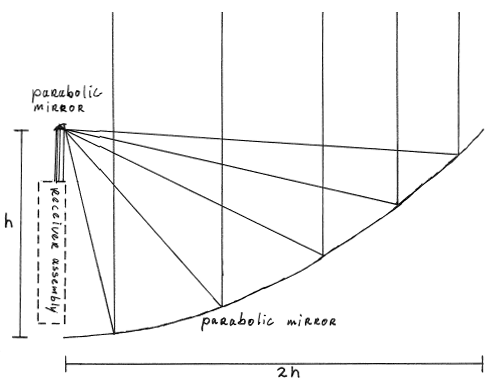
\includegraphics[scale = 0.6]{chapters/img/DiagramReceiverGeneral.png}
\caption{The diagram of the parabolic mirror}
\label{fig:diagram_Rgeneral}
\end{figure}
The draft design diagram of assembly micro lenses is shown on figure \ref{fig:diagram_Rmicrolenses} on page \ref{fig:diagram_Rmicrolenses}. The micro lenses are placed just above the \acs{SPAD} chip to focus light source on the specific pixel 2\% area. On the other hand, the micro lenses could be very heavy due to the high density of the lens material, and it also has high risk of falling off due to vibration during lunching and boosting.
\begin{figure}
\centering
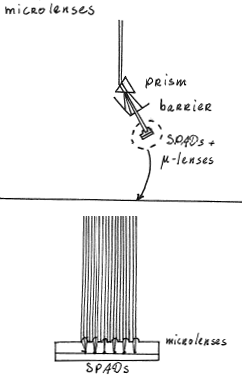
\includegraphics[scale = 0.6]{chapters/img/DiagramReceiverAssemblyMicrolenses.png}
\caption{The diagram receiver assembly micro lenses}
\label{fig:diagram_Rmicrolenses}
\end{figure}
Another way to increase the receiving efficiency is using the faceted mirror such as the figure \ref{fig:diagram_Rfaceted mirror} on page \ref{fig:diagram_Rfaceted mirror} shown. Instead of the heavy micro lenses the multi-faceted elliptical mirror can be placed to achieve the focusing. Since the faceted mirror can reach the same purpose but lighter than micro lenses, it might be a better solution after all. 

\begin{figure}
\centering
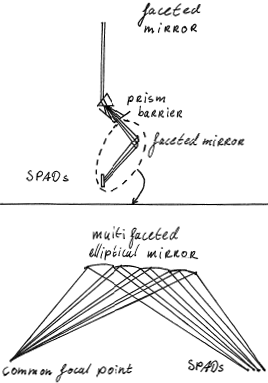
\includegraphics[scale = 0.6]{chapters/img/DiagramReceiverAssemblyFacetedMirror.png}
\caption{The diagram receiver assembly faceted mirror}
\label{fig:diagram_Rfaceted mirror}
\end{figure}


\subsubsection{Trade Criteria}
\label{TOReceiverC}
In the last paragraph, the general trade off method is elaborated but not in quantity way. It is more precise and clear to give some trade criteria to compare between options, which can be graded from 1-10 (worse to best) to indicate each criterion performance. Mass, power, volume are criteria considered as design of a constellation of micro or nano satellites. The criteria such as efficiency, reliability, resolution and \ac{FOV} are defined whether the receiver can detect photon or not and how precision it could be. Meanwhile, Cost, lifetime and availability need to be noticed generally in each subsystem.

\subsubsection{Weight Factor}
\label{TOReceiverWF}
Weight factor is given differently to each criterion due to mission objective and instrument performance requirement. Lifetime is the top objective and efficiency determines the photons can be detect or not, so both are given as maximum 10. Power, mass, volume are important since micro or nano receivers are considered. Meanwhile resolution, reliability and \acs{FOV} are also important to perform continuous accurate measurements. The mission objective is about feasibility study, so cost and availability are not the essential part.

\subsubsection{Trade summary}
\label{TOReceiverS}
The trade off table is shown in figure \ref{fig:receiver_tradeoff} on page \ref{fig:receiver_tradeoff}. The \acs{SPAD} plus micro lenses and faceted mirror designs have the much higher grades than \acs{SILAT} or \acs{MPD}. The \acs{SPAD} with micro lenses has lowest grade for efficiency, because the lenses which is manufactured in scale of micro meters can only increase the efficiency by factor of 5. On the other hand, the faceted mirror can increase the fill field from 2\% to 80\%, that is why faceted mirror has much larger efficiency. The \acs{SPAD} with faceted mirror design has the large advantages on power comsuption(100$\mu$W), mass(tens of grams) and volume($5\times5\times3[mm^{3}]$) comparing to either \acs{SILAT} or \acs{MPD}, that is much more realistic and practical if the swarm of receiver satellites are in scale of micro or even nano. 

\begin{figure}
\centering
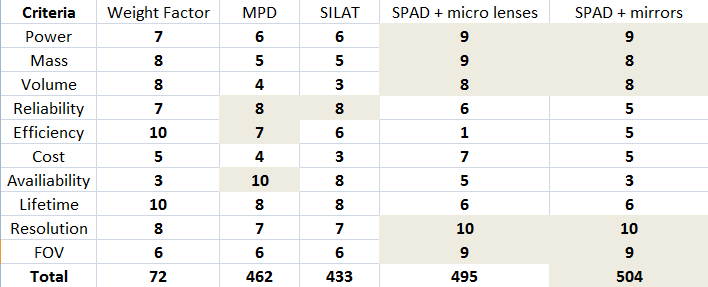
\includegraphics[scale = 1]{chapters/img/Receiver_tradeoff.png}
\caption{The receiver trade off table}
\label{fig:receiver_tradeoff}
\end{figure}
